Comme expliqué plusieurs fois précédemment, assurer la scalabilité de l'application est un point crucial de ce travail de Bachelor. En effet, l'application doit tenir la charge d'un nombre de festivaliers potentiellement important en simultané.

\section{Tests de montée en charge}

Afin de simuler un nombre important de festivaliers, il est nécessaire de mettre en place un outil permettant de simuler de réels utilisateurs. Dans la plupart des cas, ce type de test se contente de réaliser un nombre conséquent de requêtes HTTP sur l'application afin de vérifier diverses métriques. Dans le cas de \gls{beeplace}, il ne s'agirait pas d'une solution très intéressante. En effet, l'obstacle majeur à la scalabilité de l'application est la communication WebSocket, qui s'occupe de toute la synchronisation des données entres les utilisateurs. En effet, aucun appel HTTP n'est réalisé par le client vers le serveur, toute l'information transite par WebSocket. Aussi bien l'état initial du canvas que la pose d'un pixel ou encore la réception des pixels des autres utilisateurs. Il faut donc avoir cet aspect bien à l'esprit lors du choix de l'outil de test.

\subsection{Déploiement de l'application}

Afin de tester les limites de l'application sans affecter la version en production, l'application est déployée sur une seconde machine virtuelle à l'adresse suivante \href{https://dev-place.beescreens.ch}{dev-place.beescreens.ch}. Les spécifications de cette machine virtuelle sont les suivantes:

\begin{itemize}
  \item CPU 4 c\oe{}urs Intel(R) Xeon(R) CPU E5-2697 v4 @ 2.30GHz
  \item 4 Go de RAM
  \item 50 Go de disque
\end{itemize}

\gls{beeplace} est déployé sur cette machine virtuelle à l'aide de Docker et de Docker Compose. La configuration utilisée est la même que pour la version en production. Celle-ci est disponible dans le répertoire \mintinline[breaklines]{bash}{deployement/beeplace} du répertoire git.

\subsection{Choix de l'outil}

Pour pouvoir tester la communication WebSocket, il faut tester l'implémentation choisie, à savoir Socket.IO. En effet, Socket.IO utilise son propre protocole de communication~\cite{socket-io-protocol} au-dessus des WebSockets classiques, qui n'est pas forcément supporté par tous les outils de test. La documentation officielle de Socket.IO propose deux manières~\cite{socket-io-load-testing} de tester une application utilisant Socket.IO:

\begin{enumerate}
  \item Utiliser l'outil Artillery~\cite{artillery}
  \item Créer un nombre important de clients Socket.IO manuellement
\end{enumerate}

La deuxième solution n'est pas l'idéale car elle ne permet pas d'avoir des statistiques très poussées sur les performances de l'application. En effet, il est compliqué de récupérer un nombre suffisant de métriques sans finir par développer son propre outil de test. Afin de ne pas réinventer la roue, le choix initial s'est porté sur Artillery.

\subsubsection{Artillery}

Artillery propose différents moteurs utilisables pour tester une application. Il existe donc un moteur Socket.IO permettant d'avoir une solution clé en main pour tester facilement \gls{beeplace}. Les tests sont définis dans un fichier de configuration YAML, qui permet de définir les différentes phases de test ainsi que le comportement des utilisateurs virtuels (appelés scénarios). Ce fichier YAML peut importer un fichier JavaScript afin d'ajouter de la logique supplémentaire aux tests.

\begin{listing}[h]
  \inputminted{yaml}{assets/figures/artillery-test.yml}
  \caption{Test de montée en charge avec Artillery}
  \label{listing:artillery}
\end{listing}

Le test d'exemple \ref{listing:artillery} génère 1000 utilisateurs en une minute (soit environ 16 à 17 utilisateurs par seconde). Chaque utilisateur va dessiner 3 pixels aléatoirement sur le canvas et attendre ensuite 30 secondes. Cette attente est importante car le client va recevoir les pixels des autres utilisateurs pendant cette période, ce qui simule un comportement plus réaliste. La logique pour générer un pixel aléatoire ainsi que la fingerprint sont définis dans le fichier JavaScript importé \mintinline[breaklines]{bash}{functions.js}.

Cette solution très simple à mettre en place semble idéale. Cependant, un nombre important de problèmes est survenu:

\begin{itemize}
  \item Le script lance parfois une erreur \mintinline[breaklines]{bash}{Error: Callback was already called.} qui stope l'exécution du test. Plusieurs personnes semblent avoir le même problème sur \gls{github}~\cite{artillery-callback-issue} mais aucune solution n'a encore été trouvée. Utiliser un outil qui n'est pas stable n'est pas envisageable.
  \item Artillery ne permet pas de tester facilement la communication du serveur vers les clients. En effet, l'outil est plus adapté à la communication client-serveur. Ce qui est problématique afin de récupérer par exemple la configuration du canvas ou encore les pixels des autres utilisateurs.
  \item Artillery ne met pas à disposition des métriques très utiles dans ses résultats concernant les WebSockets ou Socket.IO. En effet, il n'est pas possible de récupérer la latence de la connexion WebSocket, qui est l'indicateur le plus important dans le cas de \gls{beeplace}. Artillery met à disposition une métrique \mintinline[breaklines]{bash}{socketio.response_time} qui pourrait être intéressante mais malheureusement celle-ci ne dépasse pas les 4 millisecondes, même lorsque l'application n'arrive plus à répondre, ce qui est très peu réaliste.
\end{itemize}

Ces raisons ont poussé à abandonner Artillery et à chercher une autre solution.

\subsubsection{k6}

k6~\cite{k6} est un outil de test de performance open-source écrit en Go. Il fait partie des outils de test de montée en charge les plus populaires avec plus de 20'000 stars sur \gls{github} et est utilisé par de nombreuses entreprises comme Amazon, Microsoft ou encore \gls{gitlab}. Son avantage principal dans le cas de \gls{beeplace} est que les tests s'écrivent en JavaScript (ou en TypeScript), ce qui permet encore une fois de garder une base de code commune avec le reste des applications.

k6 gère les WebSockets grâce au module expérimental \mintinline[breaklines]{bash}{k6/experimental/websockets}~\cite{k6-websockets}. Celui-ci implémente l'API WebSocket du navigateur, ce qui permet d'écrire le même code qu'habituellement. Cependant, comme discuté précédemment, Socket.IO utilise son propre protocole au-dessus des WebSockets, ce qui n'est pas pris en charge nativement par le module k6. Heureusement, un développeur a mis à disposition sur \gls{github} une implémentation de Socket.IO pour k6~\cite{k6-socket-io}. Celle-ci propose une classe \mintinline[breaklines]{bash}{K6SocketIO} permettant d'interagir bien plus facilement avec notre serveur Socket.IO.

Cette implémentation initiale n'est pas la plus aisée mais une fois mise en place, l'écriture des tests est assez concise et k6 met à disposition de nombreuses métriques lors des résultats des tests. La plus intéressante dans le cas de \gls{beeplace} est la latence de la connexion WebSocket comme discuté précédemment. Celle-ci est disponible via la métrique \mintinline[breaklines]{bash}{ws_connecting} de k6. Il est possible de vérifier que la valeur de cette métrique ne dépasse pas un certain seuil en utilisant la configuration suivante:

\begin{minted}[breaklines]{js}
  thresholds: {
    ws_connecting: [{ threshold: 'p(95)<1200', abortOnFail: true }],
  }
\end{minted}

Cet exemple de configuration permet de vérifier que 95\% des connexions WebSocket ne dépassent pas 1200 millisecondes. Si ce seuil est dépassé, le test est considéré comme un échec et s'arrête. Cela sera particulièrement utile dans la phase d'optimisation du code \ref{sec:optimisations} afin de vérifier que les changements apportés aient un impact positif sur la latence des connexions.

\subsubsection{Solution choisie}

Le choix s'est porté sur k6. Les raisons principales ont pour la plupart déjà été évoquées mais en voici un petit récapitulatif:

\begin{itemize}
  \item k6 permet une plus grande liberté dans l'écriture des tests grâce à l'utilisation d'un vrai langage de programmation (JavaScript) plutôt que d'un fichier de configuration YAML.
  \item k6 met à disposition dans ses résultats des métriques plus intéressantes pour tester la communication WebSocket.
  \item k6 est plus populaire et il est donc plus facile de trouver la documentation nécessaire pour résoudre les problèmes rencontrés.
\end{itemize}

\subsection{Implémentation du test}

\subsubsection{Types de tests}

Il est tout d'abord nécessaire de trouver quel type de test convient le mieux à la situation. La documentation k6 propose six types de tests de montée en charge:

\begin{figure}[H]
  \centering
  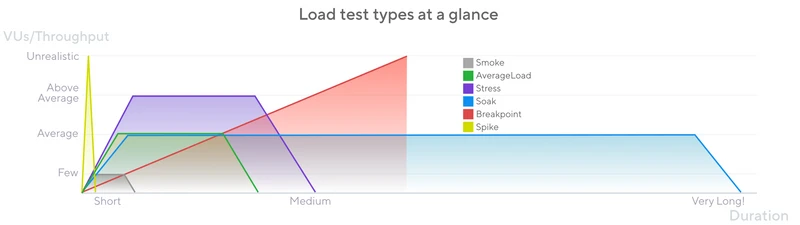
\includegraphics[width=1\textwidth]{./assets/figures/load-test-types.png}
  \caption{Types de tests de montée en charge~\cite{k6-load-test-types}.}
  \label{fig:load-test-types}
\end{figure}

\begin{itemize}
  \item \textbf{Smoke tests}: permettent de valider que le script de test fonctionne et que le système fonctionne correctement sous une charge minimale.
  \item \textbf{Average-load tests}: évaluent les performances du système dans des conditions normales prévues.
  \item \textbf{Stress tests}: évaluent les performances du système à ses limites, lorsque la charge dépasse la moyenne prévue.
  \item \textbf{Soak tests}: évaluent la fiabilité et les performances du système sur des périodes prolongées.
  \item  \textbf{Spike tests}: valident le comportement et la survie du système en cas d'augmentation soudaine, brève et massive de l'activité.
  \item \textbf{Breakpoint tests}: augmentent progressivement la charge afin d'identifier les limites de capacité du système.
\end{itemize}

TODO

\subsubsection{Architecture}

TODO

\subsubsection{Test}

TODO - ajouter code ici

\subsection{Résultats initiaux}

TODO

\section{Profiling}

TODO

\section{Optimisations}
\label{sec:optimisations}

TODO